\chapter{Role of Tropospheric Jet Changes in the Interannual Variability and Decadal Trend of Asian Monsoon Rainfall}

%%\section{to-do}
%1) May have to check how much Wang2013 beat you to the punch; Similarly, will have to take a long look at Ping Zhao's 2010 paper that provides an alternative coherent summary of SFND rainfall changes. 2) check rainfall changes between 1979-1993 and 1994-2007? 3) TRACK DOWN CITATION TO WANG H./WANG B./HUANG/DING/LEE paper on observed decadal change of the CGT in mid-70s; 4) Check Wang Hai email - useful information, either for Ch3 or 4?; 5) Inez had good way of summarizing Meiyu changes: 1) timing 2) frequency 3) intensity; 6) DING/WANG/WALLACE/BRANSTATOR PAPER should also be tracked down. 7) REALLY IMPORTANT IDEA: would be cool to look for external existing literature that talks about great heat waves/flooding episodes in some of the years included in the sample (1998 as extreme example). 8) Should really read Andrew's thesis more closely. Surely lots of references - for instance Zhang and Song 2006. 9) Figure 2 should really include a contour of the Tibetan Plateau in every figure. 10) Did you fix the stippling everywhere already?

\section{Abstract}
We have previously investigated the leading mode of July-August Asian monsoon variability (All-Asia EOF1) and argued that this mode manifests a coupling between the Himalayan Foothills and Yangtze River Valley. In this chapter, we investigate the manifestation of All-Asia EOF1 in JRA-55 reanalysis and further associated atmospheric anomalies across the Northern Hemisphere. Extreme years of All-Asia EOF1 correspond to a global-scale Northern Hemisphere wavetrain known as the Circumglobal Teleconnection (CGT), leading to robust temperature and rainfall anomalies. Geopotential height anomalies at all atmospheric levels are barotropic except for a coherent band of diabatic heating across the Himalayan foothills and Yangtze Corridor with cooling to the west, akin to the ``monsoon-desert'' mechanism. JRA-55 reanalysis supports the hypothesis in Chapter 2 that changes in moisture transport across the Yunnan Plateau cause observed rainfall anomalies. Furthermore, we propose that the pattern of diabatic heating is a direct result of these moisture transport changes, which create a robust trough and ridge pattern over East Asian high-latitudes, and therefore may contribute to the known phenomenon of phase-locking of the CGT in summer. 

Over East Asia, positive All-Asia EOF1 years feature a robust southward shift in the tropospheric jet, and vice-versa in negative years. Major late-twentieth-century changes in the latitude of frontal rainfall (the ``South Flood-North Drought'') also coincide with anomalies in East Asian jet latitude. The position of the East Asian jet responds to variability in heating over China, but we argue that the jet also translated global climate change into regional impact over East Asia. Though the mid-latitudes force East Asian monsoon weather chaotically (the ``Silk Road'' pattern), the effect of twenty-first-century global warming on the East Asian jet and on moisture transport across the Yunnan Plateau can be studied and projected with greater confidence. Anticipating changes in these two elements of Asian summer climate may improve projections of twenty-first-century rainfall change in China and East Asia, which remain highly uncertain as of the latest International Panel on Climate Change report (IPCC5).

\section{Introduction}

%%KEY INTRO PARAGRAPHS?
% 1) The monsoons are the key mechanism that delivers rainfall to the tropics and subtropics. Countless studies attempt to explain their variability in terms of external forcing, including any number of oscillations...

	The global monsoon dictates a substantial fraction of the world's hydrologic budget. Typically, rainfall is delivered to monsoonal regions in abundance within a narrow seasonal window. In Asia, the timing, duration and severity of monsoon rainfall determines whether agriculture in the region will be fruitful for the year or will succumb to drought or flooding. As a result, countless efforts have been made to prognosticate its totals and associate them to exterior modes of variability, such as ENSO, ... and ... . Some success has been made, but proper projections are likely impossible due to chaos, especially in the mid-latitudes where forecasting cannot surpass weather forecasting range by much \citep{Teng2013}.
	
% 2) Particularly key: Existing predictions of Asian monsoon climate changes are weak and potentially unfounded!
	This lack of predictability is especially problematic because even small changes in the mean state of the monsoon may impact the lives of over 4 billion people. Unfortunately, the highly heterogeneous terrain of the South and East Asian monsoons produce computational challenges that few models can resolve adequately. The IPCC5 suite of models provides no consensus on changes in the East Asian monsoon. Even this limited conformity between individual models should be viewed with skepticism. They are designed with many different types of performance objectives in mind, and may not perform well over the Asian monsoon region. Furthermore, aquaplanet versions of these models produce completely different patterns of response in future under even elementary perturbations due to the inability of models to adequately parametrize moist convection and cloud formation \citep{Stevens2013}. We suggest that the way forward lies in our knowledge of the dynamics particular to the Asian monsoon, and key components whose changes we can project.

% 3) In this chapter we investigate the role of the tropospheric jet as a potential intermediary that translates global forcing into local impacts. As the edge of the monsoon circulation, responds to changes in monsoon, but also clearly influenced by extra-tropical storminess. The jet is probably uniquely responsible in the climatology of the East Asian monsoon and its variations due to the unusual configuration of the subtropical monsoon. 
	In this work, we focus on the role of the tropospheric jet as an intermediary between global warming and regional response. At a theoretical level, the tropospheric jets marks the poleward boundaries of the Hadley Cells, and shift equatorward in summer and poleward in winter forced by insolation \citep{Bordoni2008}. A growing body of regional literature also emphasizes the importance of the shifting in Hadley Cell in regulating the inter-hemispheric energy differential. Thus, the tropospheric jet is already known to be shifting in response to forcing from global warming.

% 4) locally, the jet may take on particular importance to the South Asian and East Asian monsoon
	In East Asian summer, the jet plays an important role both in shaping the climatological distribution of rainfall and in transporting storms. The passage of the tropospheric jet north of the Tibetan Plateau summer is a precondition for the onset of the South Asian monsoon \citep{Yin1949,Yeh1959,Hahn1975}. In East Asia, a positive feedback with the Tibetan Plateau forces high-amplitude standing waves in the jet that in turn create favorable conditions for convection over China \citep{Yang2002,Molnar2010,Chen2015}. Global climate anomalies are thereby translated into unusual local weather\citep{Nigam1989,Broccoli1992,Park1997}. The jet also serves as a waveguide for storms propagating from the Eurasian interior via the ``Silk Road'' teleconnection \citep{Hoskins1993,Ambrizzi1997,Kosaka2012}. The unusually strong meridional temperature gradients in East Asia, which exist because of the presence of the Tibetan Plateau, allow for storms to propagate across much longer distances than other regions with weaker temperature gradients \citep{Branstator2002}. It is also well-known from past research that shifts in the jet's latitude and strength change patterns of storminess and rainfall in East Asia \citep{Liang1998,Branstator2002,Kwon2007,Du2009,Li2014}.  Given the interconnections between jet position and climate anomalies in Asia, if global warming has forced a jet shift, this could force changes in the mean or variability of the Asian monsoon.
	
% (may have to distinguish between subtropical jet and POLAR jet - see range of papers that discuss these two separately.
	 
	 %5) The jet should register changes in monsoon variability between years, and may also INFLUENCE its variability. We pursue this argument to its fullest extent and propose hypotheses for the future of the Asian monsoon. There may be also be local changes in the monsoons that influence the jet. 
	Given the observed interaction between the East Asian jet and Asian monsoon climatology, we expect that anomalies in each time series are also interrelated. We seek to prove two objectives: 1) That the leading mode of July-August rainfall variability, hereafter All-Asia EOF1 \citep{Day2015} also corresponds to shifts in the tropospheric jet; 2) That the South Flood-North Drought also corresponded to \nth{20}-century changes in the East Asian tropospheric jet. By associating jet changes with the leading mode and decadal trend of Asian monsoon rainfall, we may improve skill in the prediction of \nth{21}-century changes in Asian rainfall from anticipating the future of the tropospheric jet. To date even simplified models have struggled to produce consistent depictions of future changes in world climate and rainfall. By synthesizing existing literature on the future of the jet with our findings, we suggest the potential future in the variability of the East and South Asian monsoons.
	  
	%IDEA: the jet serves as a two-way intermediary between regional and global variability.
	-3 independent issues: timing, intensity and northward extent. timing being both beginning and the end, when the jet goes away. SST changes could change intensity, 
	
\section{Methods}

\subsection{JRA-55 Reanalysis}

	We rely on the JRA-55 reanalysis product assembled by the Japanese Meterological Association (JMA). JRA-55 is a state-of-the-art 56-year (1958-2013) reanalysis product whose fields are calculated at a model resolution of up to 640x320 (.625$^{\circ} \times .625^{\circ}$), with exact number of longitude points varying by latitude. The products used in this analysis are upscaled to 1.25$^{\circ} \times 1.25^{\circ}$. Model levels at 700, 500 and 200 hPa were used, as well as column-integrated values where relevant. Composites of the five most positive and negative years of both All-Asia EOF1 and All-Nepal Monsoon Rainfall are produced for each of these fields. 
	
	%%need to introduce relevant cites and also indicate data retrieval times and such
	
\subsection{Historical Precipitation and Temperature Records}

	; 2) GPCC;

	Monthly temperature anomalies from 1958 to 2013 gridded at $1^{\circ}$ by $1^{\circ}$ resolution were obtained from the Berkeley Earth Surface Temperature project, freely available at \url{http://www.berkeleyearth.org/data/} \citep{Rohde2012}. BEST agrees closely with past historical temperature estimates, but the gridless methodology used can incorporate a wider range of temperature records \citep{Rohde2013}. According to their best estimate, global land mean temperature increased by $.89 \pm .06^{\circ}$C from 1950-1959 to 1990-1999. Therefore, in order to compare local temperature anomalies on an even footing, the temperature time series are detrended based on 1958-2013 local slope. At each point, we separate the time series into 12 separate monthly time series (each consisting of 56 Januarys, Februarys and so on) and then detrend each monthly time series based on the 56-point trend in that month.
	
\subsection{Composite Analysis}		
	
	Separate composite anomalies were produced using the five most positive years of All-Asia EOF1 and five most negative years \citep{Day2015}. We also repeated the same procedure with the five most positive and negative years of All-Nepal Monsoon rainfall. Further detail is included in Tables \ref{tab:t41} and ~\ref{tab:t42}. In most figures in our paper, we show the difference between positive and negative composites of relevant fields, except where otherwise specified. In July, our positive composite consists of the years
	
\subsubsection{Montecarlo Estimates of Statistical Significance}	
	
	We calculate the statistical significance of differences between positive and negative composites both analytically and via a Montecarlo method with 10,000 iterations. The analytical approximates the distribution of anomalies as Gaussian. In each iteration, we create random non-overlapping positive and negative composites of five random years each from any of the 56 Julys (and analogously for August) and take their difference. A $p$-value is obtained at each spatial point by comparing that point to our database of 10,000 potential alternative composites. The Montecarlo method is generally found to be a stricter test of significance and is used to mark statistical significance in figures. We also calculate the probability that the \textit{area} exceeding a 95\% confidence level could be obtained at random. When this value is calculated, we delimit the region of interest on relevant figures and list the $p$-value on the top-right of the figure.

\subsection{Jet Count Density} 

	\citet{Schiemann2009} constructed a data set of jet `counts' in the Tibetan Plateau region (46$^{\circ}$ E-130$^{\circ}$ E, 17$^{\circ}$ N-58$^{\circ}$ N) from ERA-40 reanalysis for 1958-2001, where a count is defined as any local maximum in zonal wind with westerly magnitude greater than $30$ m s$^{-1}$; further details can be found in section 2 of \citet{Schiemann2009}. We show daily mean jet latitude averaged across $90-130^\circ$E in Figure ~\ref{fig:jet_seasonal}a and monthly anomalies in Figure ~\ref{fig:jet_seasonal}b and c. Results are not sensitive to the choice of longitude range. Figure ~\ref{fig:climo} presents contours of jet frequency estimated by a kernel density method, which estimates a probability distribution from a set of discrete data observations. The \citet{Schiemann2009} database is also tested for covariance with the Rainband Detection Algorithm (RDA) catalog from Chapter 3 ~\ref{fig:jet_seasonal}.
	
\section{Composites of All-Asia EOF1 in JRA-55}

\subsection{Circumglobal Teleconnection}

	We build composites of the most positive and negative years of All-Asia EOF1 and find robust global change in upper-tropospheric height (Z200) across the Northern Hemisphere. The largest signal is a massive rise in geopotential height in the Tropics in the July composite, a known phenomenon in strong ENSO years ~\ref{fig:cgt_zonal}, even though All-Asia EOF1 is not significantly correlated with ENSO. The absolute magnitude of anomalies in the Tropics remains less than in mid-latitudes because its variability is much lower (sidebar of Figure ~\ref{fig:cgt_zonal}a). To focus on wavelike mid-latitude behavior, we subtract the zonal mean anomaly in subsequent figures where useful, as shown for instance in Figure ~\ref{fig:cgt_zonal}c and ~\ref{fig:cgt_zonal}d.
	
	In July (Figure ~\ref{fig:cgt_z}a), strong All-Asia EOF1 years are associated with a zonal wavenumber 5 standing wave spanning the entire Northern Hemisphere. Analyzing 200-mb geopotential height (Z200),  pronounced positive lobes are visible over Russia, the eastern Pacific, western North America and the Azores, and negative lobes over Pakistan, northeast Asia and northern Europe. In August (Figure ~\ref{fig:cgt_z}b), a similar pattern is obtained with some shifts: the northeast Asian lobe bifurcates into a Korean and Aleutian pair, the Siberian high strengthens and the North American high merges with that in the Eastern Pacific. Both the July and August Z200 anomaly patterns are significant at a 95\% confidence level. Considering the mid-troposphere and near-surface, we find that geopotential height anomalies are mostly barotropic and remain visible at the 700-mb level, except for over Pakistan where the 200-mb low is replaced by a surface high, and a belt from the eastern Tibetan Plateau eastward with 200-mb highs and 700-mb lows. These reflect cooling over Pakistan and heating over northern India, the Yangtze River Valley and western Pacific. All patterns are significant at a 95\% level except for Z700 in August.
	
	These patterns strongly resembles the Circumglobal Teleconnection (hereafter CGT) studied in \citet{Ding2005a}. \citet{Branstator2002} originally found that, in regions of strong meridional temperature gradient such as East Asia, a pattern with zonal wavenumber 5 can extend around the globe, with the tropospheric jet serving as a waveguide favoring the zonal propagation of storms. They were able both to find evidence of such a mode in reanalysis and demonstrate its existence in a simplified model. Figure 1c of \citet{Branstator2002} closely resembles our Figure ~\ref{fig:cgt_zonal}d. Looking more closely at Figures 5b and c of \citet{Ding2005a} we find that they are practically identical to our Figures ~\ref{fig:cgt_z}a and ~\ref{fig:cgt_z}b (with sign inverted), including the set of changes between July and August. Furthermore, geopotential height anomalies of the studied global wavetrains in both \citet{Branstator2002} and \citet{Ding2005a} are consistently barotropic except over India ~\ref{fig:cgt_z}. We conclude that the mid-latitude wavetrain associated with All-Asia EOF1 and the CGT as defined by \citet{Ding2005a} are the same pattern.
	
	Another way of displaying the same wavetrain pattern is to consider the upper-level meridional wind (V200). Since the zonal mean of meridional wind is 0 \citep{Ding2007} and also near-zero in composites, waves are apparent without additional filtering. Figure ~\ref{fig:cgt_v} shows V200 for the July and August composites. The number of lobes can easily be counted, and the July wavetrain appears to be of wavenumber 6 while August is of wavenumber 5. From the Aleutian Islands to the eastern United States, the pattern of meridional wind anomalies in fact reverses from July to August, while remaining largely similar over Eurasia, showing substantial change between July and August. The existence of substantial differences between the July and August wavetrain patterns was also found in \citet{Ding2005a}. Although \citet{Day2015} argues that July and August All-Asia EOF1 are highly similar over the Asian monsoon region, this is evidently not true at the global scale.

%%% PARAGRAPH ON PREDICTIVITY OF ALL-NEPAL MONSOON RAINFALL - probably not strong enough to be included, unnecessary.	
%	In \citep{Day2015}, we discussed the potential of All-Nepal Monsoon Rainfall (ANMR) as representative of All-Asia EOF1-type variability. Here we show that ANMR has some predictive power on CGT-type patterns. Using a different set of composite years chosen as extreme years of All-Nepal Monsoon Rainfall (Table ~\ref{tab:t42}), we repeat the process in Figure ~\ref{fig:cgt_z} for July (several years overlap with peak All-Asia EOF1 years). In August, only a faint CGT pattern is found (not shown), so it may be more reasonable to suggest that the CGT and All-Nepal Monsoon Rainfall are both driven by the same external variability.  
		
%% NEED A PARAGRAPH DISCUSSING HOW JRA-55 COMPOSITES SUPPORT HYPOTHESIS FROM CHAPTER 2 - also just need to expand description of figures included, let them do the work.
\subsection{Regional Changes Associated with All-Asia EOF1}

\subsubsection{Moisture Transport Across the Yunnan Plateau}

	We examine the regional dynamics within the Asian monsoon that potentially drive All-Asia EOF1-type variability. Furthermore, we can assess whether the hypothesis in \citet{Day2015}, that changes in moisture transport across the Yunnan Plateau couple the Himalayan Foothills and Yangtze River Valley, is borne out in JRA-55 reanalysis. JRA-55 surpasses its predecessors in model resolution and may therefore be more credible.
	
	We consider the distribution of diabatic heating within the South and East Asian monsoons associated with All-Asia EOF1. The column-integrated heating $Q$ is calculated according to JRA-55 as the residual of the sum of total column upwelling and downwelling short-wave fluxes $\Delta R_S\uparrow$ and $\Delta R_S\downarrow$, upwelling and downwelling long-wave radiative fluxes $\Delta R_L\uparrow$ and $\Delta R_L\downarrow$, sensible heat flux from the surface  $\Delta SH_{sfc}$ and latent heat flux  $\Delta LH=L \dot P$, all provided as monthly products in JRA-55:
	
\begin{equation}
	Q=R_{S_{top}\downarrow}-R_{S_{sfc}\downarrow}-R_{L_{sfc}\downarrow}-R_{S_{top}\uparrow}+R_{S_{sfc}\uparrow}-R_{L_{top}\uparrow}+R_{L_{sfc}\uparrow}+SH_{sfc}\uparrow+LP
\end{equation}
	
	$L$ is the latent heat of condensation of water vapor.
	
	Panels ~\ref{fig:cgt_dyn}b-d focus on the Asian monsoon region (10$^{\circ}$E-170$^{\circ}$W and 5$^{\circ}$N-50$^{\circ}$N) and only show composite differences that are statistically significant. All three panels reveal a coherent belt of anomalies stretching from the Himalayan Foothills eastward to the Yangtze River Valley. The Himalayan Foothills and western half of the Yangtze River Valley moisten significantly, associated also with a low-level westerly wind anomaly. The general spatial distribution matches the known Indian summer monsoon dipole between the Himalayan Foothills and Monsoon Zone. A significant easterly wind anomaly is also found in northern China. Panel d shows that the precipitable water content also rises on the southeastern corner of the Tibetan Plateau. Again, this matches the spatial distribution of rainfall changes with All-Asia EOF1 found in \citet{Day2015} and suggests changes in water vapor transport as culprit.
	
	In arid northwestern India, the low-level westerly anomaly leads to significant drying of near-surface air. Figure ~\ref{fig:cgt_700} suggests that the, in spite of being next to the Arabian Sea, depends on moisture transport from the Bay of Bengal for its moisture. In strong negative All-Asia EOF1 years the Monsoon Zone of Central India receives, and we
	
	In negative All-Asia EOF1 years there is no mean ascent over western India, whereas in positive years conditions favor ascent (Figure  ~\ref{fig:cgt_500}b).
	
	In the case of panel Figure ~\ref{fig:cgt_dyn}d we have not include the positive and negative composite estimates separately because they are rather similar to each other. During the positive composite the magnitude of southward water vapor transport northward in southern China is up to 250 kg m$^{-1}$ s$^{-1}$, but only about 170 kg m$^{-1}$ s$^{-1}$ in negative years with essentially none across the Yunnan Plateau.  In addition, the eastward moisture transport in positive composite years across the Yunnan Plateau is roughly 100 kg m$^{-1}$ s$^{-1}$, and practically zero in negative composite years. Therefore, moisture transport across the Yunnan Plateau seems to be contributing significantly to the anomalously strong southerly monsoon flow in southern China. JRA-55 composite analysis strongly supports the hypothesis that changes in moisture transport across the Yunnan Plateau are integral to the variability of All-Asia EOF1.
						
	In fact, JRA55 reanalysis suggests that low-level winds reverse from westerly to easterly in August between positive and negative All-Asia EOF1 years (not shown). Nonetheless the overall pattern of inter-composite differences in low-level wind anomalies and specific humidity at 700-mb is very similar between July and August. This is also true of panel 5d, where the pattern of change in vertical velocity is is very similar. Unsurprising given how All-Asia EOF1 is selected, but still indicative of correlation between increased low-level water vapor and uplift.
			
	Looking at the positive and negative composites of vertical velocity (Figure ~\ref{fig:cgt_500}), it is clear that the biggest change is a continuous band of ascent spanning from the Yunnan Plateau across the Yangtze River Valley and to Japan. We can also see major chances in arid western India (Gujarat vicinity), which switches from no ascent to strong mean ascent, possibly explaining the high amplitude of All-Asia EOF1 in that location. In Negative Composite years, Southeast Asia and the southern Bay of Bengal feature considerably more ascent. All of these changes are significant according to Figure ~\ref{fig:cgt_dyn}c.
	
\subsubsection{Meridional Shift of the East Asian Jet}

	Over East Asia, Figure ~\ref{fig:cgt_u} reveals that the inter-composite difference between positive and negative All-Asia EOF1 years is locally reflected as a \textit{robust southward shift of the jet} visible in both July and August. We further explore the connection of the jet and East Asian monsoon variability subsequently across the rest of the year. d
	
\subsection{Can the East Asian monsoon force the CGT?}

	The source of CGT-type variability has been debated in the literature. The Himalayan Foothills and Yangtze River Valley are seen to be a region of diabatic heating. However, this does not gurantee that the Indian Monsoon is driving the CGT pattern. \citet{Ding2007} investigated the daily evolution of a Eurasian wavetrain pattern bearing strong resemblance to the CGT. In their estimation, the original forcing lies in the region of the North Atlantic jet exit, a region of very high variability in geopotential height. The downstream propagation of signals from this region then controls active and break spells in the Indian monsoon, equivalent to forcing India EOF1 positively or negatively. The diabatic heating from the Indian monsoon then further strengthens the Central Asian high, which in turn can trigger a Siberian high that brings anomalous rainfall to North China. Here We suggest that our hypothesis of moisture transport linking the Himalayan Foothills to the Yangtze River Valley \citep{Day2015} is not incompatible with their theory - our mechanism and theirs could be mutually reinforcing.

	...However, a reasonable counter-argument is that the precursors of Indian monsoon variability are not visible as propagating waves because Tropical variability is influenced by different processes such as the Madden-Julian Oscillation.

	...At a more fundamental level, this also means that the topography of the Yunnan Plateau influences the Asian monsoon's forcing of the CGT. 
	
	NEW ARGUMENT: The phase locking of the CGT in summer is the function of both the pattern of diabatic heating from the distribution of All-Asia EOF1 as well as the TOPOGRAPHY, which sets particular allowed configurations of the jet by conservation of potential vorticity.

	We present a different view from \citet{Ding2007}, in that we suggest that the ultimate trigger is the internal variability of the Indian monsoon which shifts its preferred path of moisture transport between Central India and the Himalayan Foothills. When moisture is transported to the Himalayan Foothills, a downstream coupling results with the potential to generate a full CGT-type circulation. The advantage over Ding and Wang is that it can explain dynamically why the monsoon is stimulated by CGT - in fact the monsoon is providing its own forcing through its inherent variability. \textcolor{red}{The particular spatial distribution of All-Asia EOF1, and ultimately the geometry of the Yunnan Plateau, encourage the phase-locking of the Circumglobal Teleconnection in summer (as opposed to winter, when there is no preferred phase).} 

\section{East Asian Jet Shifts and the ``South Flood-North Drought''}

	In the previous section, we showed that positive and negative All-Asia EOF1 years are reflected as zonally-continuous southward and northward shifts of the East Asian Jet extending into the northwestern Pacific Ocean. The relation of East Asian jet latitude and rainfall in July and August leads us to investigate a link between jet position and rainfall in other seasons, using the Rainband Detection Algorithm (RDA) Catalog established in Chapter 3. It has been argued in the past that the meridional shift of the jet is simply a local response to heating patterns in the troposphere \citep{Yu and Zhou}. However, the hemispheric mean latitude of the tropospheric jet also reflects the poleward boundary of the Hadley Cell \citep{Kang2015}, and may generally be influenced by modes of global and extratropical variability. Therefore, it is reasonable to suggest that exterior forcing may alter the position of the jet, and therefore change the pattern of rainfall in East Asia. We do not suggest that the jet exclusively forces the position of rainbands in China, but rather that there may exist a mutual feedback. In the following text, we reveal a close connection of jet and rainfall position in China throughout the Meiyu progression, and also coupled historical change in both (the ``South Flood-North Drought'').
	
\subsection{Climatology of the East Asian Jet}

	The East Asian jet is closely associated with the five rainfall stages of East Asian monsoon rainfall described in Chapter 3. Beginning in May, the East Asian jet moves from its winter position on the southern flank of the Tibetan Plateau to a summer latitude well north of the plateau.  A full monthly jet climatology is visible in \citet{Schiemann2009}; During this transition, the jet occupies intermediate configurations that correspond to different stages of China rainfall (Figure ~\ref{fig:climo}). Peak rainfall rates in China from May to mid-July corresponds to the months when the climatological latitude of the jet impinges on the Tibetan Plateau, because the interaction of the tropospheric jet and Tibetan Plateau strengthens convergence and rainfall downstream over China and the western Pacific Ocean \citep{Molnar2010,Sampe2010,Chen2014}. From May to September,  the climatological latitude of rainfall, rainbands and jet density are all closely coupled, with peak jet density occurring 5 to 10 degrees north of the latitude of peak rainfall. This agrees with the prediction that, in a region of strong frontal conditions as observed in East Asia, the co-occurrence of a strong upper-tropospheric jet and a coupled equatorward region of ascent and strong rainfall \citep{Holton2004}. 
	
	The initiation of the Pre-Meiyu corresponds roughly to the beginning of the jet's northward passage. During Meiyu season, the preferred latitude of the jet continues to shift northward. The period of frequent double rainband occurrence during the Post-Meiyu corresponds to the jet's maximal northward extent. Finally, the jet returns southward during the Fall Rains in October and November, which produces only a weak rainfall response.
	
	In addition, Figures ~\ref{fig:climo}a-e show mean rainfall, jet frequency and rainband position during each stage, as well as their zonal average (sidebars). From the Pre-Meiyu to Post-Meiyu, each northward jump in peak rainband frequency corresponds to a similar shift in jet count density, with a southward offset of about 5 degrees.
	
\subsection{Jet Changes, 1980-2001 Versus 1958-1979}

	In Figure ~\ref{fig:jet_seasonal}a, we show the zonal average over $90-130^\circ$E) of mean jet latitude, averaged over the years 1958-1979 (blue solid line) and 1980-2001 (dashed red line) with 95\% confidence intervals overlain. Both significant changes in rainband statistics described in the previous section correspond to southward shifts in mean jet latitude. During the Pre-Meiyu (May), the tropospheric jet is shifted southward by almost 2$^{\circ}$ in 1980-2001 relative to 1958-1979, when its mean latitude was $\approx 41^{\circ}$N. We estimate the significance of this change using a two-tailed Kolmogorov-Smirnov (K-S) test. Since the K-S test requires that all samples are independent, we first remove temporal autocorrelation due to synoptic variability by assimilating daily mean jet latitude into 4 day blocks. A subsequent K-S test finds that the shift is significant with $p=0.003998$. During the Post-Meiyu (days 201-273), when a southward shift in rainband latitude is found in 1980-2001 relative to 1958-1979, the mean latitude of the jet is also consistently displaced southward. We assimilate daily mean jet latitude into 7-day blocks before performing a K-S test, and find a $p$-value of this shift of $p=0.05667$.
	
\section{Hypothesis}

	The Meiyu front and tropospheric jet covary in latitude from May to September in the climatological mean, and parallel changes are found in rainband attributes and mean jet latitude between 1951-1979 and 1980-2007. Therefore, the South Flood-North Drought appears to reflect an alteration in jet dynamics. We propose that both the Pre-Meiyu decline in rainband frequency and the Post-Meiyu southward shift of rainband latitude result from a single phenomenon: an overall southward displacement of the jet's summer progression over East Asia. In climatology, the Pre-Meiyu corresponds to both a surge in rainfall and the beginning of the jet's northward transit, when its preferred latitude begins to impinge on the Tibetan Plateau. We propose that the observed southward shift in the jet during May has delayed the date when the jet first impinges on the Tibetan Plateau, resulting in a delay in Pre-Meiyu onset and prolonged Spring Rain conditions. This is manifested as weaker rainfall and decreased rainband frequency in central China in May. Subsequently, we argue that the reduced northward extent of the jet during the Post-Meiyu has shifted rainfall and mean rainband latitude southward. Finally, we suggest that the southward displacement of the summer jet cycle results in a decrease in northern China annual rainfall and an increase in central China annual rainfall, producing a South Flood-North Drought response. Thus, our hypothesis can explain the major observed changes in rainfall and rainband statistics during the Pre- and Post-Meiyu as well as cumulative yearly change.
	
	To test our hypothesis, we investigate the relation of interannual anomalies in jet latitude and rainband properties. Figure ~\ref{fig:jet_seasonal}b shows a scatter plot of rainband \textit{frequency} anomalies versus jet latitude anomalies in May (days 121-150). Most years with a decrease in rainband frequency feature a southward jet shift, and vice-versa, and such years occur mostly during 1980-2007. A similar relation is found between monthly anomalies in rainband \textit{latitude} and jet latitude during July-August (days 201-260, Figure ~\ref{fig:jet_seasonal}c). In the latter figure, we exclude rainbands south of 28$^{\circ}$ N from calculated anomalies, since such rainbands reflect South China Sea storms, rather than jet influence \citep{Day2015}. Together, Figures ~\ref{fig:jet_seasonal}b and ~\ref{fig:jet_seasonal}c suggest that interannual changes in jet latitude affect Pre-Meiyu rainband frequency and Post-Meiyu rainband latitude.
	
	 %%should probably move away from previous conclusion that jet shifts caused SFND, because causality difficult to distinguish - but, still reasonable to suggest that we can get more predictive skill on the monsoon by understanding future jet changes.
	 	 
	We propose that the delayed passage of the jet to the north of the Tibetan Plateau has shortened the Pre-Meiyu season, decreasing May rainfall in central China, and restricted the northward advance of precipitation, consequently reducing Post-Meiyu rainfall in northern China. This interpretation is a modern analog of the ``Jet Transition Hypothesis'' described in \citet{Chiang2015}, wherein East Asian rainfall changes on paleoclimate timescales are ascribed to modulation in the seasonal cycle of the tropospheric jet. 	
 		 
\section{Potential for Constrained Projection}

\subsection{Key Argument}
	%% KEY ARGUMENT
	Causality is difficult to distinguish. The different elements of the Asian monsoon must shift in physically consistent manner, but this does not reveal the initial trigger. The jet changes in the SFND may indeed be simply a local response to patterns of diabatic heating. Nonetheless, we suggest that the historical association between them means that \textit{we can constrain the sample space of future changes in the Asian monsoon by predicting future changes in the jet}.
	
\subsection{Historical trends in the jet}
	%historical jet changes
	Observations show that the global annual mean latitude of the tropospheric jet has shifted poleward, in tandem with tropospheric heating and lower-stratospheric cooling in the mid-latitudes, increased subtropical static stability, and the expansion of the Hadley circulation \citep{Fu2006,Archer2008,Fu2011}. Opposite trends are found in some regions and the variation by season is significant; we find that the East Asian portion of the jet has shifted equatorward, in agreement with past studies \citep{Yu2007, Archer2008}. Recent work proposes that the observed southward displacement of the jet over the Pacific Ocean was caused by \nth{20}-century changes in tropical Pacific convection and SST \citep{Park2014a}. Thus, the global poleward trend in jet latitude and the East Asian equatorward shift are compatible observations that reflect the heterogeneous spatial distribution of \nth{20}-century warming.

\subsection{Future changes}
\subsubsection{CMIP5 consensus}
	%IPCC5 consensus paragraph - kinda boring, so keep short. should list the caveats of CMIP5 talks
	\citet{Lee2014} analyzed \nth{21}-century changes in a suite of CMIP5 models and concluded that the robust stabilization of the atmosphere in almost all models would tend to decrease the variability associated with the CGT. However, these models may suffer from the fundamental issue of being targeted to hit the mean, and therefore not exploring a suitable range of unlikely scenarios. The state of future projections for the Asian monsoon is highly uncertain. The ability of many models out of IPCC to simulate basic features of the South and East Asian monsoon remains in question.

\subsubsection{Idealized studies}
	%Consensus about the future jet from modeling work'
	The poleward expansion of the Hadley Cell is projected to continue under \nth{21}-century warming \citep{Frierson2007,Lu2007,Kang2012}, but a recent study predicts that anomalous \nth{21}-century heating of the eastern Pacific Ocean will drive the Pacific jet further equatorward \citep{Park2014}.
		 
\section{Conclusion}

	The existence of a Circumglobal Teleconnection in the Northern Hemisphere was only demonstrated and modeled in the past several decades. Its proper resolution depends on having sufficiently powerful global climate models. With the refinement in resolution of JRA-55 we are now resolving All-Asia EOF1 accurately and also showing its association to global climate. In the past, two potential drivers of the CGT were proposed: The Atlantic jet, where variability is highest, and the Indian monsoon, where the anomalies are baroclinic rather than barotropic and diabatic heating occurs. Modeling studies show that heating across the Northern Hemisphere can all force a global wavetrain-type pattern, so we are not forced to choose a singular locus as driver. Nonetheless, we propose here a third driving region - the diabatic heating along the Yangtze River Valley, which produces a diagonally tilted trough-ridge pattern over China and Siberia. In turn, since we propose that the diabatic heating reflects changes in moisture transport, we therefore propose that the topography of the Yunnan Plateau leads to phase-locking of the CGT, not directly by deflecting upper tropospheric circulation, but rather controlling patterns of diabatic heating in the Asian monsoon.
	
	Composite analysis with JRA-55 also suggests that high-resolution reanalysis products feature changes in moisture transport across the southeastern Tibetan Plateau. In particular, positive and negative All-Asia EOF1 years in JRA-55 feature a change in Yangtze River moisture source, from a sizable Bay of Bengal component to being predominantly sourced from the South China Sea. This should also be visible in present-day isotopic records in that region - since the transport distance from the Bay of Bengal to the Yangtze River is long, we would expect water vapor with a Bay of Bengal origin arriving in China to be depleted, and that positive All-Asia EOF1 years should see negative excursions in Yangtze River $\delta ^{18}$O records. This is also a region where many speleothems are located, cave stalagmites featuring tends of thousands of years of continuous deposition from which a continuous time series of $\delta ^{18}$O can be extracted. Traditionally, speleothem $\delta ^{18}$O records are viewed as proxies of local monsoon intensity. However, recent work increasingly argues that East Asian speleothem records such as Hulu and Sanbao are primarily a record of changes in the Indian monsoon upstream that are then transported downwind \citep{Cai2015,Pausata2011,Baker2015}. Proving that changes in water vapor transport from the Bay of Bengal alter the \textit{present-day} isotopic signature in central China would support the new swath of reinterpretation of speleothems.

	We have shown that a significant amount of the annual and decadal variability in Meiyu front activity is accompanied by changes in the westerly jet. Two major changes in the progression of the East Asian summer monsoon were previously reported: 1) A decrease in frequency during the Pre-Meiyu season (days 121-160, May 1-June 9; $p=.0019$); and 2) A southward shift in rainband latitude during the Post-Meiyu season (days 201-273, July 20-Sep 30; $p=.0003$). The latter change is responsible for the South Flood-North Drought trend in total yearly rainfall. In addition, both time periods display a southward anomaly in mean jet latitude during 1980-2007 relative to 1951-1979. We argue that both Pre-Meiyu and Post-Meiyu changes in rainfall and rainband statistics are caused by a southward shift of the summer progression of the East Asian tropospheric jet. In particular, we propose that the delayed passage of the jet to the north of the Tibetan Plateau has shortened the Pre-Meiyu season, decreasing May rainfall in central China, and restricted the northward advance of precipitation, consequently reducing Post-Meiyu rainfall in northern China. This interpretation is a modern analog of the ``Jet Transition Hypothesis'' described in \citet{Chiang2015}, wherein East Asian rainfall changes on paleoclimate timescales are ascribed to modulation in the seasonal cycle of the tropospheric jet. 	
 
	Many components of our results have been presented in previous work. \citet{Xuan2011} find a southward shift in the jet and increased Yangtze Valley rainfall in July. \citet{Yu2004} and \citet{Yu2007} found a southward shift in July-August jet latitude and suggested a link with the South Flood-North Drought. Potential mechanisms for late \nth{20}-century East Asian climate change include changes in Indian Ocean SST \citep{Qu2012}, decreased sensible heating from the Tibetan Plateau \citep{Liu2012a,Hu2015} and aerosol forcing \citep{Song2014}.
	
 By linking the South Flood-North Drought to changes in the seasonal advance of the tropospheric jet, we open the possibility of projecting \nth{21}-century East Asian rainfall change by improving our understanding of the effect of further global warming on the regional and global behavior of the tropospheric jet.
	
	%%VERY LAST PARAGRAPH - ANY INTUITION ON THE FUTURE OF THE SFND?
	
	We suggest a preliminary answer to the question of what will happen to the South Flood-North Drought pattern of rainfall change in China, as well as future changes in All-Asia EOF1.

	
\section{Acknowledgments}

	Significant portions of the current work were produced in collaboration with Jacob Edman and John Chiang and under the guidance of Inez Fung. The formula for column-integrated heating was retrieved from \url{http://ds.data.jma.go.jp/gmd/jra/atlas/en/D_HEATcol.html}.


\newpage	
\clearpage	
\section{Tables and Figures}

%%%% TABLES %%%%

%% TABLE 4.1 - LIST OF YEARS USED IN POSITIVE AND NEGATIVE COMPOSITES OF ALL-ASIA EOF1	
\begin{table}[p]

\caption{Years used for the positive and negative composities of All-Asia EOF1 in July (July AA+ and AA-) and August (August AA+ and August AA-), expressed in units of standard deviation. Years are chosen as the most extreme values of All-Asia EOF1 as previously published in \citet{Day2015}.}
\centering

\begin{tabular}{ c c c c}
	 	 		\multicolumn{2}{c}{All-Asia EOF1 Composites} 	&			Years				&		Value (Std. Devs.)			\tabularnewline	
				\hline
	 \multirow{2}{*}{July} 		&  +							&	1970, 1987, 1998, 2002, 2007 	&	1.65, 2.25, 1.47, 1.35, 1.62		\tabularnewline
	 						&  -							&	1959, 1973, 1976, 1978, 1994       &	-1.59, -1.25, -1.45, -1.40, -2.65	\tabularnewline
	 \multirow{2}{*}{August}	&  + 							&	1958, 1965, 1993, 1998, 2005	&	1.85, 1.77, 2.00, 2.67, 1.49		\tabularnewline
	 						&  -  							&	1973, 1978, 1984, 1994, 2006	&	-1.96, -2.04, -1.68, -1.64, -1.40 \tabularnewline

\end{tabular}
\label{tab:t41}
\end{table}

%% TABLE 4.2 - LIST OF YEARS USED IN POSITIVE AND NEGATIVE COMPOSITES OF ALL-NEPAL MONSOON RAINFALL	
\begin{table}[p]

\caption{Years used for the positive and negative composities of July All-Nepal Monsoon Rainfall (July N+ and N-) and August All-Nepal Monsoon Rainfall (August N+ and August N-) expressed in units of cumulative rainfall (also translated into standard deviation. Years are chosen as the most extreme values of ANMR between 1961-2007, during which APHRODITE features high-quality station coverage \citep{Day2015}.}
\centering

\begin{tabular}{ c c c c}
	 	 		\multicolumn{2}{c}{Nepal Composites} 	&			Years				&			Monthly Rainfall (mm)		\tabularnewline	
				\hline
	 \multirow{2}{*}{July} 		&  +						&	1984, 1985, 1988, 1998, 2007 	&	14.45, 13.45, 14.52, 13.51, 13.67		\tabularnewline
	 						&  -						&	1971, 1973, 1991, 1993, 2006       &	9.04, 8.23, 8.12, 9.17, 9.16 			\tabularnewline
	 \multirow{2}{*}{August}	&  + 						&	1961, 1962, 1966, 1988, 1998	&	12.47, 13.45, 11.88, 12.38, 13.83		\tabularnewline
	 						&  -  						&	1972, 1984, 1986, 2004, 2006	&	6.62, 7.32, 7.82, 7.41, 7.78			\tabularnewline

\end{tabular}
\label{tab:t41}
\end{table}

\newpage
\clearpage

%%%% FIGURES %%%%


%% FIGURE 4.1 - Composite geopotential height anomalies with and without zonal mean
\begin{figure}
\centering
\noindent\includegraphics[width=42pc]{Figures/ch4/CGT_1}
\caption{a) July composite difference in 200-mb level geopotential height (Z200) between positive and negative All-Asia EOF1 years. Sidebar: Zonal mean of composite anomaly. b) July Z200 composite anomaly expressed as Z-score (units of local std. devs.), showing massive anomaly in the Tropics. c) July Z200 composite anomaly with zonal mean removed, highlighting mid-latitude wavetrain. d) Same as Panel c, but expressed as Z-score as in panel b.}
\label{fig:cgt_zonal}
\end{figure}

%% FIGURE 4.2 - Geopotential height anomalies in upper troposphere, middle troposphere and lower troposphere (200mb, 500mb and 700mb)
\begin{figure}
\centering
\noindent\includegraphics[width=42pc]{Figures/ch4/CGT_2}
\caption{July All-Asia EOF1 composite difference in a) Z200, c) Z500 and e) Z700. Panels b, d and f are analogous to panels a, c and e except with procedure repeated for August. Local statistically significant differences at a 95\% level are marked by stippling. $p$-values at the top-right of each plot show the likelihood via Montecarlo testing that the \textit{amount of statistically significant area} between 20$^{\circ}$N and 65$^{\circ}$N (delimited on figures) could be achieved at random (given by $1-p$). A value above .95 indicates statistical significance at a 95\% confidence level.}
\label{fig:cgt_z}
\end{figure}

%% FIGURE 4.3 - July composite 200-mb meridional wind (V200 anomalies)
\begin{figure}
\centering
\noindent\includegraphics[width=36pc]{Figures/ch4/CGT_3}
\caption{Composite anomalies in 200-mb meridional wind (V200) in a) July and b) August, both of which show a robust global mid-latitude standing wave. As explained in Figure ~\ref{fig:cgt_z} and in main text, $p$-values shown at top-right indicate statistical significance of entire pattern between 20$^{\circ}$N and 65$^{\circ}$N}
\label{fig:cgt_v}
\end{figure}


%%% MOST LIKELY ANOTHER FIGURE COMING IN HERE: GLOBAL DISTRIBUTION OF TEMPERATURE AND RAINFALL IMPACTS


%% FIGURE 4.4 - Series of additional plots suggesting dynamics of CGT
\begin{figure}
\centering
\noindent\includegraphics[width=42pc]{Figures/ch4/CGT_5}
\caption{Ffith CGT plot}
\label{fig:cgt_dyn}
\end{figure}

%% FIGURE 4.5 - Positive and negative composites of low-level specific humidity and winds
\begin{figure}
\centering
\noindent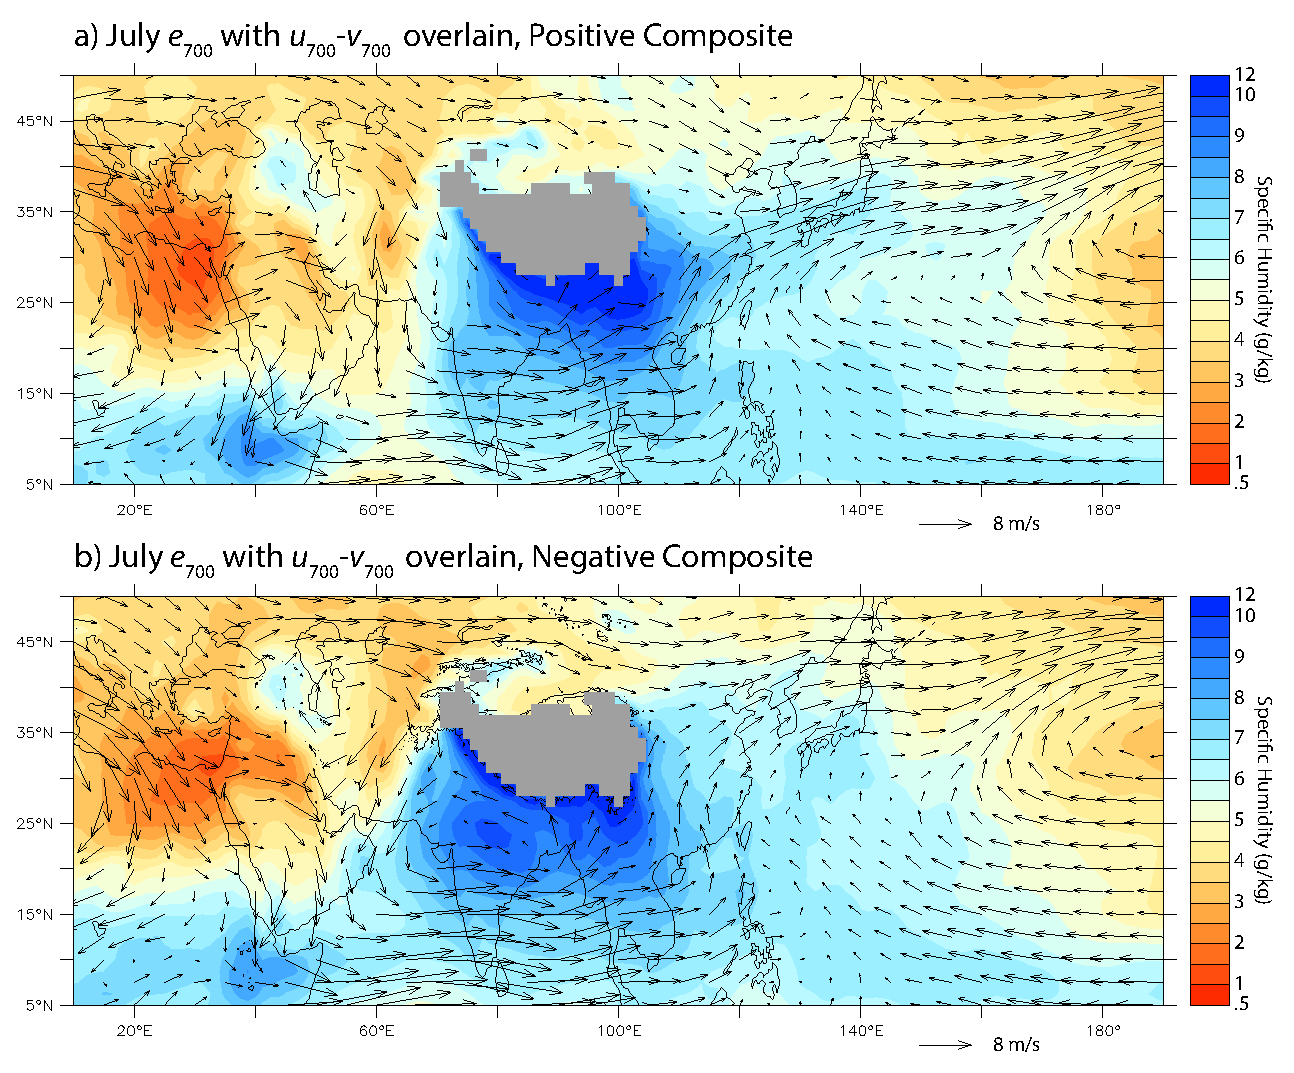
\includegraphics[width=36pc]{Figures/ch4/CGT_6}
\caption{Sitxh CGT plot}
\label{fig:cgt_700}
\end{figure}

%% FIGURE 4.6 - Positive and negative composites of mid-tropospheric ascent and winds
\begin{figure}
\centering
\noindent\includegraphics[width=36pc]{Figures/ch4/CGT_7}
\caption{Sventh CGT plot}
\label{fig:cgt_500}
\end{figure}

%% FIGURE 4.7 - All-Asia EOF1 variability looks locally like a jet shift.
\begin{figure}
\centering
\noindent\includegraphics[width=42pc]{Figures/ch4/CGT_4_alt}
\caption{Frouth CGT plot}
\label{fig:cgt_u}
\end{figure}

%% FIGURE 4.8 Climatology of rainfall stages including rainfall, jet and most likely rainband configuration, and longitudinal averages.
\begin{figure}
\centering
\noindent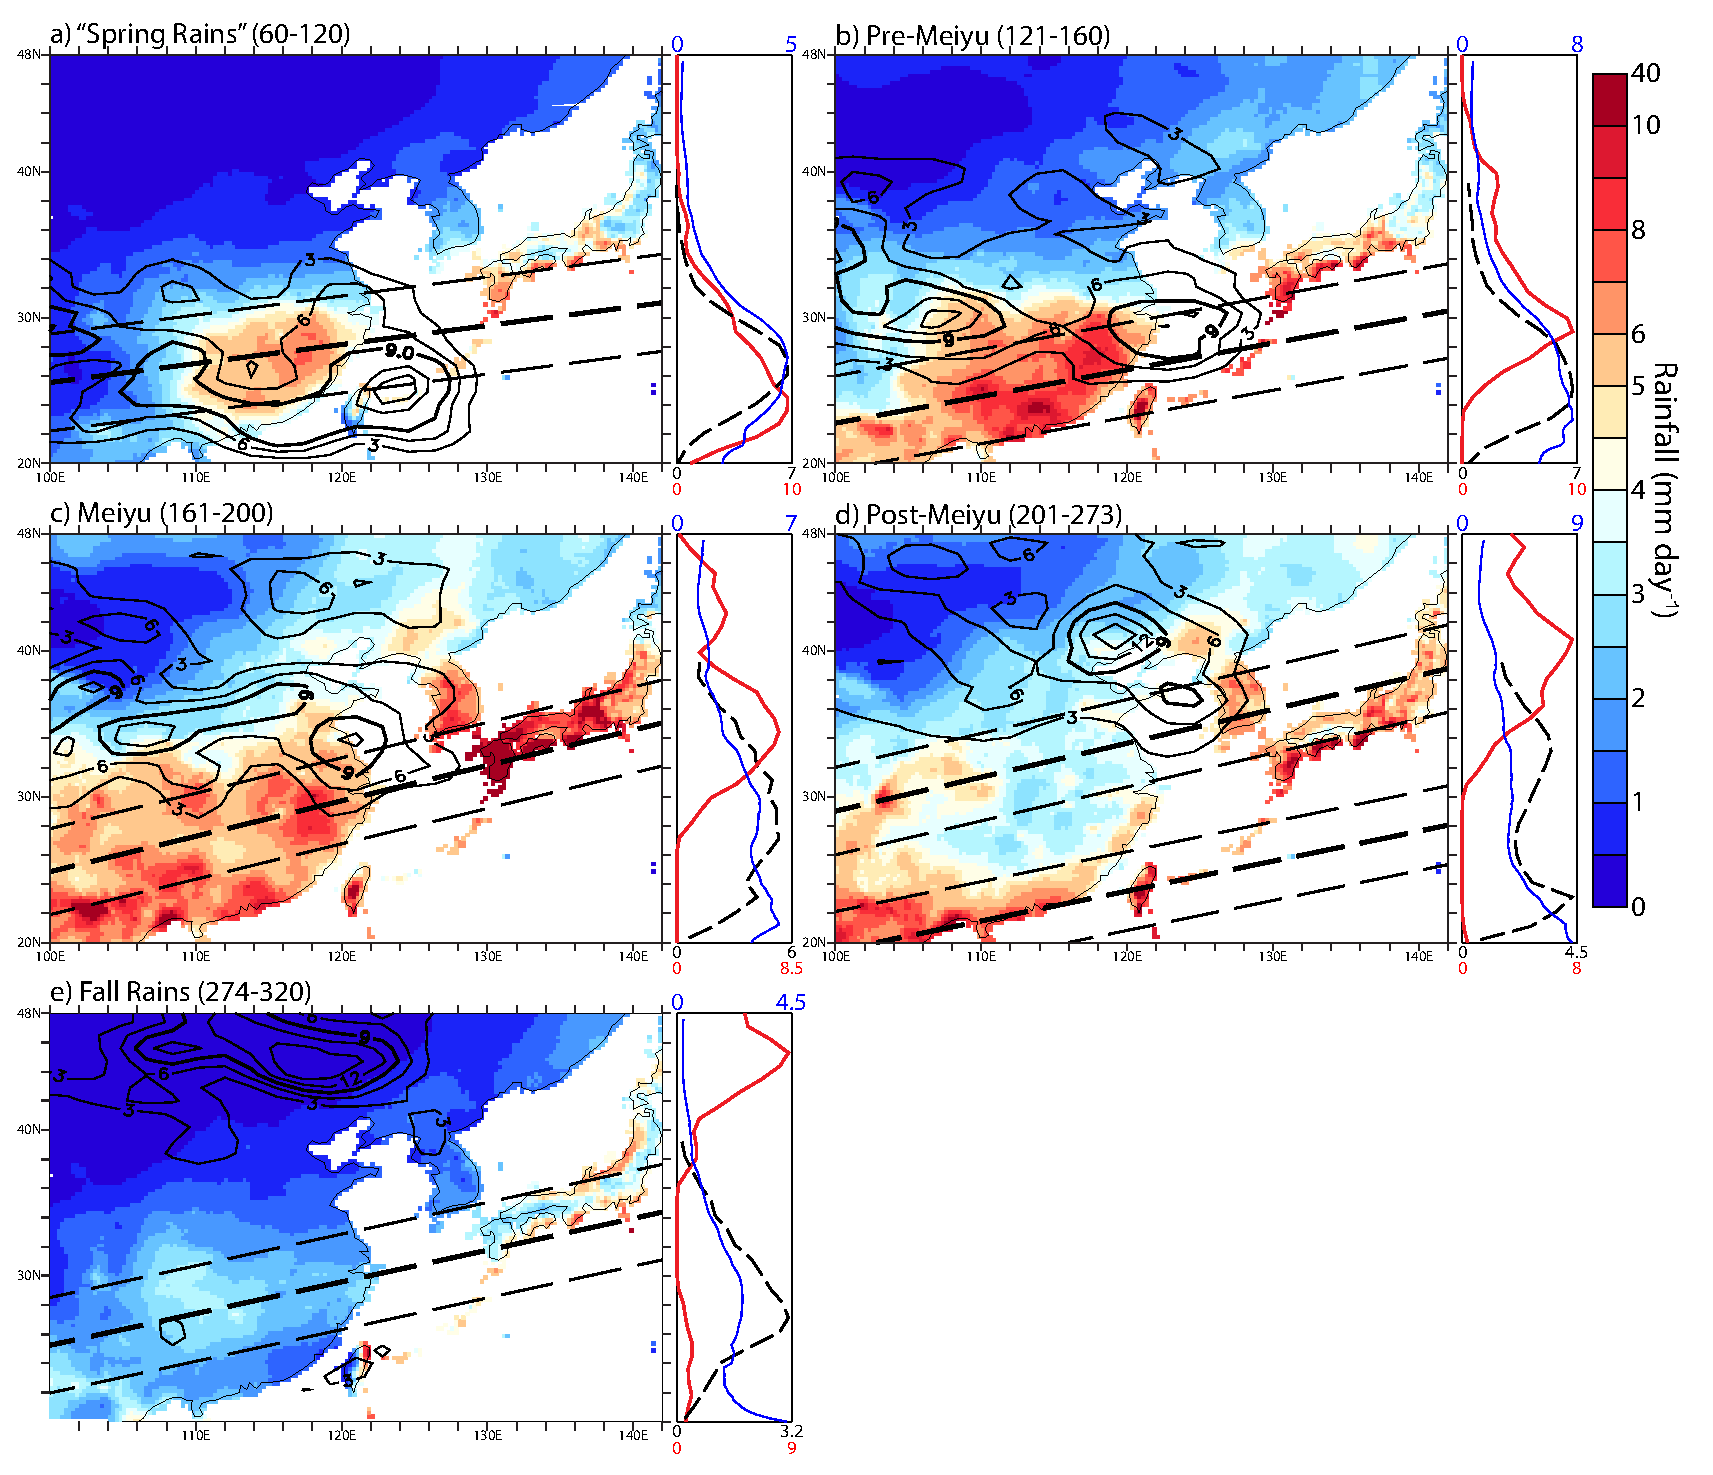
\includegraphics[width=36pc]{Figures/ch4/climo}
\caption{Climatology of East Asian rainfall stages showing rainfall (shading), jet kernel density (contours of probability density in units of $10^{-4}$) and most common rainband position during that stage. Sidebars shows, for each time period, the longitude average over 105-123$^{\circ}$E of rainfall (thin blue line, units of mm day$^{-1}$), jet kernel density (red line, units of $10^{-4}$) and rainband position (dashed black line, absolute probability in \%, 1-degree latitude smoothing). From the Pre-Meiyu to Post-Meiyu, a peak in preferred jet latitude consistently occurs 5 degrees north of a corresponding maximum in rainband frequency.}
\label{fig:climo}
\end{figure}


%% FIGURE 4.9 - 2D spatial distribution of change showing a) full year b) Pre-Meiyu and c) Post-Meiyu
\begin{figure}
\centering
\noindent\includegraphics[width=36pc]{Figures/ch4/changes_2d_jet}
\caption{a) Whole year mean rainfall change, showing the South Flood-North Drought pattern; b) Rainfall changes during the Pre-Meiyu (days 121-160) with contours of jet density change overlain; c) Same as c, but for the Post-Meiyu (days 201-273). Statistical significance at 95\%/99\% level overlain with single/double hatches. Sidebars show, for each time period, the longitude average over 105-123$^{\circ}$E of changes in rainfall (thin blue line, units of mm day$^{-1}$), jet kernel density (red line, units of $10^{-4}$) and rainband position (dashed black line, absolute probability in \%, 1-degree latitude smoothing).}
\label{fig:changes_2d}
\end{figure}

%% FIGURE 4.10 - Changes in jet mean between 1951-1979 and 1980-2007 + scatter plots of jet and rainband monthly anomalies.
\begin{figure}[htbp]
\centering
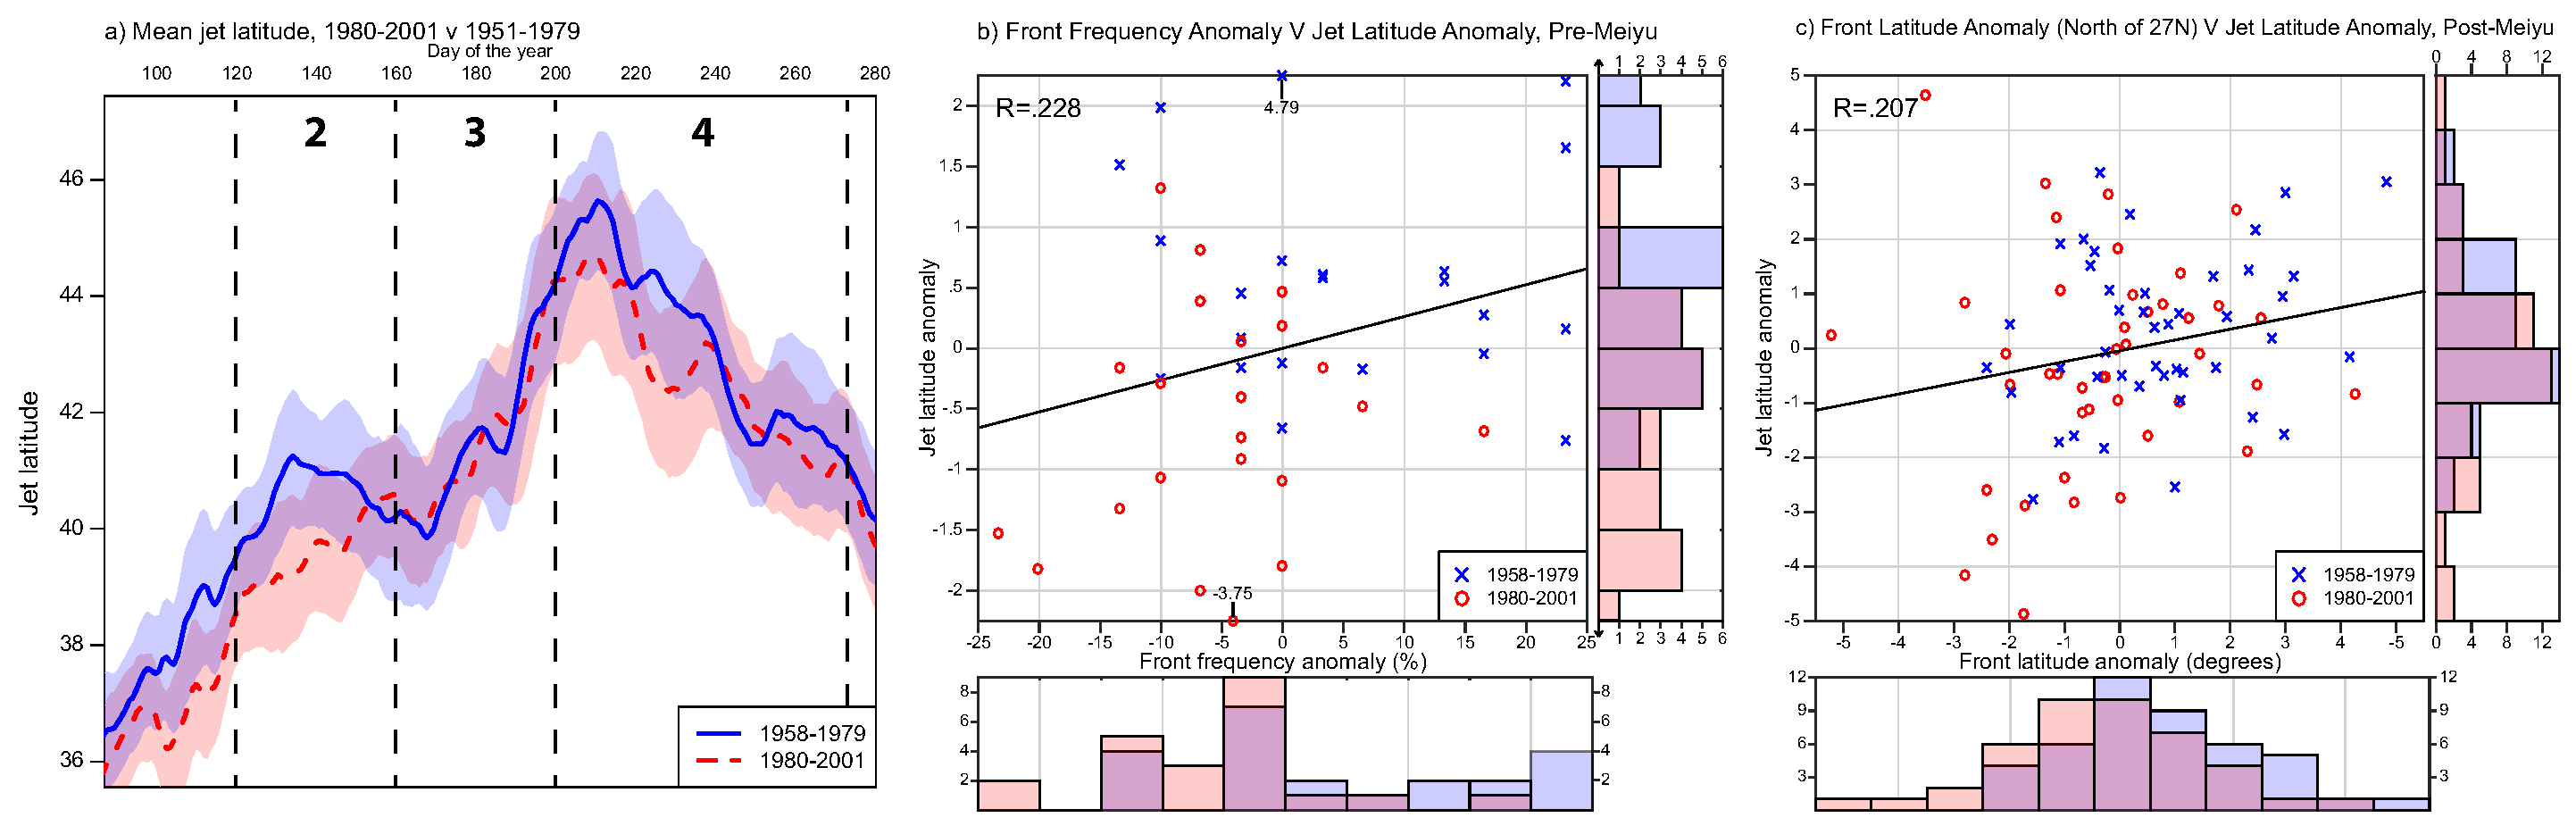
\includegraphics[width=42pc]{Figures/ch4/jet}
\caption{a) 7-day running mean latitude of the westerly jet in the region 90-130$^\circ$E for the years 1958-1979 (blue, solid) and 1980-2001 (red, dashed). Bootstrapped 95\% confidence intervals are shaded. Time periods: 2 - Pre-Meiyu; 3 - Meiyu; 4 - Post-Meiyu; b) Plot of monthly anomalies in rainband frequency versus monthly anomalies in jet latitude during days 121-150 (May) for 1958-1979 (blue X) versus 1980-2001 (red circle); c) Same as b), but showing 30-day anomalies of rainband latitudes during the Post-Meiyu (201-230 and 231-260, each set of 30 days treated as a separate point). Histograms of anomalies are also shown on the side of each figure.}
\label{fig:jet_seasonal}
\end{figure}

%% FIGURE 4.11 - Temporal autocorrelation of the jet used to demonstrate the choice of block size for averaging.
\begin{figure}[htbp]
\centering
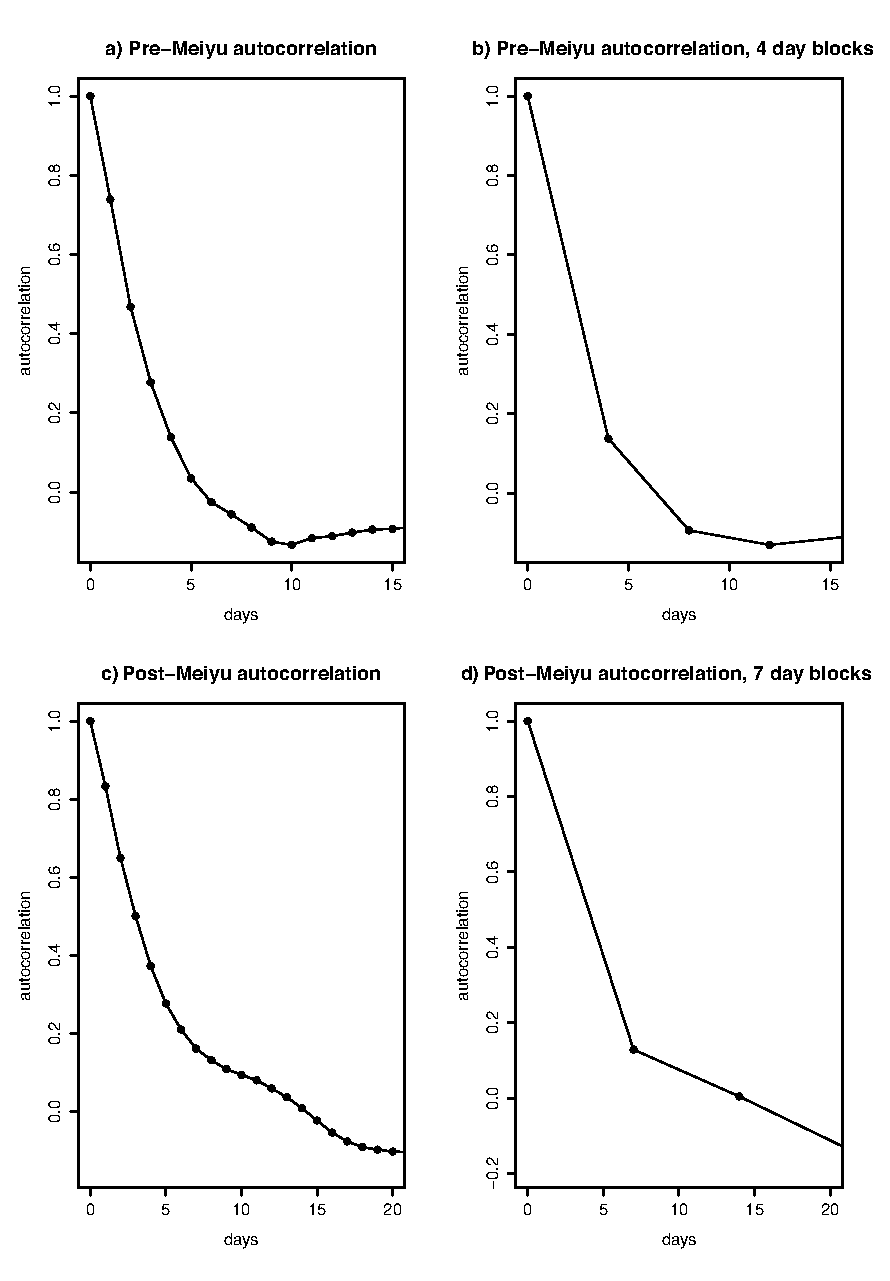
\includegraphics[width=24pc]{Figures/ch4/jet_autocorr}
\caption{The accumulation of the jet into blocks eliminates the autocorrelation from the daily mean latitude signal. During the Pre-Meiyu, mean daily jet latitude is further smoothed over 4 days (panels a and b); During the Post-Meiyu, we average over 7 days (panels c and d).}
\label{fig:jet_autocorr}
\end{figure}
